\section{Fundamentação Conceitual}
\label{fundamentacao}


\subsection{Paradigma Publish/Subscribe}

O paradigma \textit{Publish/Subscribe} (Pub/Sub) é um modelo de comunicação assíncrona em que produtores (\textit{publishers}) publicam eventos em canais lógicos, enquanto consumidores (\textit{subscribers}) recebem mensagens associadas aos tópicos de seu interesse. Diferentemente do modelo cliente-servidor tradicional, esse padrão promove desacoplamento entre emissores e receptores.\cite{microsoft_pubsub}

A comunicação é mediada por um intermediário responsável por distribuir eventos aos assinantes adequados, favorecendo escalabilidade e comunicação reativa em sistemas distribuídos, além de reduzir o acoplamento entre componentes e evitar dependências diretas típicas de modelos síncronos, que podem comprometer a flexibilidade e a resiliência do sistema.

No NATS, esse paradigma é implementado por meio de \textit{subjects}, tópicos hierárquicos utilizados para o roteamento eficiente das mensagens.


\subsection{NATS Core}

O NATS Core corresponde à camada básica de mensageria do ecossistema NATS e implementa comunicação leve baseada no paradigma \textit{publish/subscribe}. Seu modelo prioriza simplicidade, baixa latência e alto throughput, oferecendo comunicação nativa muitos-para-muitos (M:N) entre processos distribuídos.

Além do paradigma pub/sub discutido anteriormente, o NATS Core incorpora mecanismos como \textit{request-reply}, para interações do tipo requisição-resposta, e \textit{queue groups}, que permitem distribuir mensagens entre consumidores e balancear carga de processamento.

No que se refere à confiabilidade, o NATS Core opera com semântica \textit{at-most-once}, em que a mensagem é enviada sem persistência nativa ou retransmissão automática, priorizando desempenho e caracterizando o modelo básico de entrega da plataforma.

\subsection{JetStream}
Complementando o modelo básico do NATS Core, o JetStream introduz persistência e streaming, ampliando as garantias de entrega da plataforma.

Por meio de \textit{streams} e \textit{consumers}, permite armazenamento de mensagens, replay de eventos e desacoplamento temporal entre produtores e consumidores, possibilitando que mensagens sejam consumidas mesmo após sua publicação. Além disso, suporta semânticas de entrega \textit{at-least-once} e cenários \textit{exactly-once} baseados em confirmações de processamento.

Segundo a documentação oficial do NATS, o JetStream também suporta replicação baseada em quorum via algoritmo RAFT, fornecendo tolerância a falhas e alta disponibilidade em ambientes distribuídos \cite{nats_jetstream}.

\section{Arquitetura da Tecnologia NATS}
\label{fundamentacao}


\subsection{Componentes}
\label{fundamentacao}
O ecossistema NATS é estruturado a partir de três componentes centrais:

\begin{itemize}

\item \textbf{NATS Server (\textit{nats-server})}: núcleo responsável por gerenciar conexões, realizar o roteamento das mensagens e manter o estado das assinaturas ativas. Sua arquitetura é orientada a baixa latência e processamento eficiente de eventos.

\item \textbf{Clients (Publishers e Subscribers)}: aplicações que interagem com o servidor publicando ou consumindo mensagens. No protótipo desenvolvido, o \textit{publisher} representa o serviço emissor de eventos, enquanto os \textit{subscribers} representam os consumidores dessas respostas.

\item \textbf{Subjects}: tópicos hierárquicos utilizados para endereçamento e roteamento das mensagens (por exemplo, \textit{investimentos.acoes.petr4}). A entrega é baseada no interesse dos assinantes registrados nesses subjects.

\end{itemize}

\subsection{Modelo de Comunicação}
\label{fundamentacao}
O middleware adota um modelo de comunicação assíncrono baseado em troca de mensagens.

\begin{itemize}

\item \textbf{Publish-Subscribe (1:N):} mensagens publicadas em um \textit{subject} são entregues aos assinantes interessados e ativos no momento da publicação, caracterizando o modelo básico de comunicação do NATS.

\begin{figure}[ht]
\centering
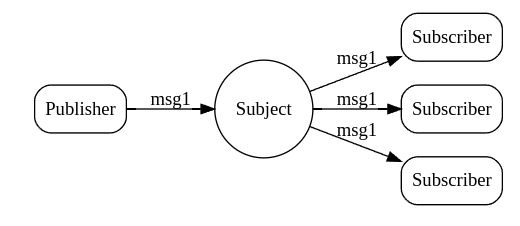
\includegraphics[width=0.75\linewidth]{figs/pubsub.png}
\caption{Modelo Publish-Subscribe no NATS.}
\label{fig:pubsub}
\end{figure}

\item \textbf{Request-Reply (1:1):} padrão construído sobre pub/sub em que um cliente envia uma requisição e recebe resposta por meio de um \textit{reply subject}, viabilizando comunicação orientada a serviços.

\begin{figure}[ht]
\centering
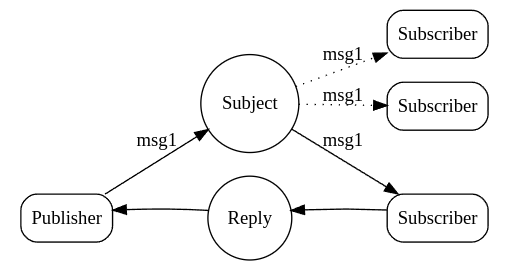
\includegraphics[width=0.75\linewidth]{figs/request-reply.png}
\caption{Modelo Request Reply.}
\label{fig:request-reply}
\end{figure}

\item \textbf{Queue Groups:} múltiplos consumidores compartilham uma mesma assinatura, mas cada mensagem é processada por apenas um deles, permitindo balanceamento de carga e escalabilidade horizontal.

\begin{figure}[ht]
\centering
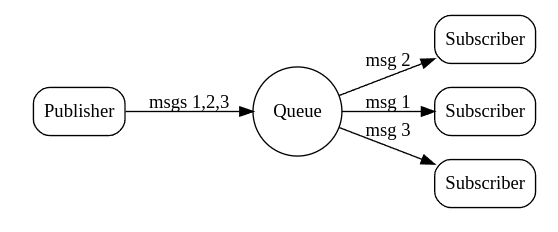
\includegraphics[width=0.75\linewidth]{figs/queue-groups.png}
\caption{Modelo Queue Groups.}
\label{fig:queue-groups}
\end{figure}

\end{itemize}

\subsection{Subjects}

Os \textit{subjects} são os identificadores utilizados pelo NATS para organizar e direcionar a comunicação entre clientes, funcionando como canais lógicos de publicação e subscrição. Esse modelo garante transparência de localidade, já que produtores e consumidores não precisam conhecer a localização uns dos outros.

Eles podem ser estruturados de forma hierárquica por meio do caractere \texttt{.} (\textit{ponto}), permitindo organizar tópicos do mais genérico ao mais específico, como em \texttt{orders.created}. Essa hierarquia é essencial para o roteamento eficiente das mensagens.

O NATS também suporta \textit{wildcards} em subscrições: \texttt{*} (\textit{asterisco}), que representa exatamente um nível da hierarquia, e \texttt{>} (\textit{maior que}), que corresponde a múltiplos níveis subsequentes. Essa flexibilidade permite implementar estratégias como filtragem de mensagens, controle de acesso e otimização do roteamento.

\subsection{Roteamento das mensagens}

O NATS adota um modelo de roteamento baseado em interesse (\textit{interest-based routing}), no qual os servidores mantêm um grafo dinâmico de \textit{subscriptions} \cite{nats_faq}. Esse grafo representa os \textit{subjects} de interesse dos clientes e é propagado entre os nós do cluster. Quando uma mensagem é publicada, ela é encaminhada apenas para os servidores que possuem assinantes interessados no \textit{subject} correspondente, evitando \textit{broadcast} desnecessário e aumentando a eficiência do sistema.

